\section{Steady state spectroscopy}
\label{sec:SSS}

\subsection{Structural influences}

In the following, the steady state spectra for ZnTPP and ZnOEP in the two solvents toluene (Tol) and benzonitrile (BN) are analyzed.

First, we are comparing the spectra of the two different materials ZnTPP and ZnOEP as depicted in \cref{fig:ZnTPPZnOEP}. The measured data is in great accordance with 
literature \cite{Wagner.1994}.
\begin{figure}[h]
    \centering
    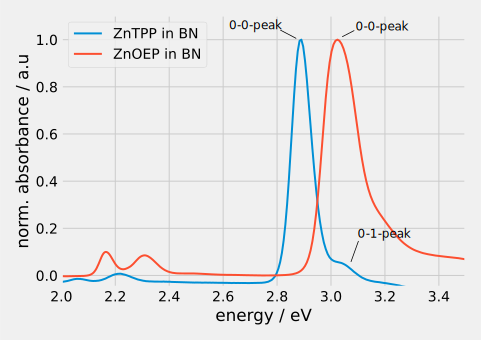
\includegraphics[width = 12cm]{Program/ZnTPPZnOEP.pdf}
    \caption{UV / VIS spectrum of ZnTPP and ZnOEP in benzonitrile.}
    \label{fig:ZnTPPZnOEP}
\end{figure}
The peak positions are analyzed using \textit{scipy.optimize.curve\_fit()}. The absorption spectrum consists of four bands in our detected range. The Soret band $S_\mathrm{2}$ (B-band) of ZnTPP peaks at 
\SI{2.89 \pm 0.01}{\eV}, while the weaker band at \SI{3.05\pm0.03}{\eV} can be assigned to a convolution of transitions of vibrational bands \cite{Even.1982}.
The two bands in the in the range of of 2 to \SI{2.4}{\eV} are the Q-bands. 

For ZnOEP the Sorbet peak occurs at \SI{3.03\pm 0.02}{\eV}. This gives clear blue shift compared to ZnTPP.
This shift in the peak position can be explained by investigating the structure of the the two molecules. As shown in (ref), ZnTPP differs structurally from ZnOEP by having four benzene rings.
These enlarge the system of conjugated $\pi$-bonds, which leads to a lowering of the absorption energy\cite{Kohler.2015}. Intuitively, we can
understand this by imagining the system of conjugated bonds as a box as often treated in quantum mechanics.
Therefore it seem plausible that enlarging the box lowers the energy levels.

\subsection{Influence of solvent}

It is well-known that the choice of solvent during UV/VIS spectroscopy can significantly affect the position of absorption \cite{Parson.2015}. This phenomenon can be attributed to several factors. Firstly, the solvent molecules undergo reorganization around the target molecule as it transitions from the ground state to the excited state, resulting in changes in symmetry and charge distribution. Secondly, the conformation of the molecule itself can be influenced by the solvent.
\begin{figure}[h]
    \centering
    \includegraphics[width = 13cm]{Program/ZnTPPinBNTol.pdf}
    \caption{UV/VIS absorbance spectrum in two different solvents: benzonitrile and toluene}
    \label{fig:ZnTTPdiffrentSolvents}
\end{figure}
A straightforward example to illustrate this point is a nonpolar chain of carbon atoms. In a polar solvent, the chain tends to coil up since it experiences fewer interactions with the surrounding solvent molecules. On the other hand, in a nonpolar solvent, the chain may stretch out, exhibiting a more planar backbone.

In our specific case, the absorption peak for ZnTPP in toluene was observed at \SI{2.8917 \pm 0.0001}{\eV}. However, when ZnTPP  is in solution in benzonitrile, the absorption peak shifted to \SI{2.932297\pm0.000001}{\eV}.

% The fact that the choice of solvent during UV / VIS spectroscopy changes the position of the absorption is well known\cite{Parson.2015}. There are multiple effects, changing the positions such as reorganisation of 
% the solvent around the molecule when the molecule performs a transitions from the ground state to the exited state as the symmetry and charge distribution changes. Furthermore, the conformation
% of the molecule can change with the choice of solvents. A easily understandable example would be the a nonpolar chain of carbon atoms. In a polar solvent, this chain would form a coil as it would have less interaction with 
% the solvent whereas in a nonpolar solvent it might stretch out and show a more planar backbone. 
% In our case the peak for ZnTPP in toluene was \SI{2.8917 \pm 0.0001}{\eV}, whereas for ZnTPP in benzonitrile peaks at \SI{2.932297\pm0.000001}{\eV}. 

% \begin{figure}[h]
%     \centering
%     \includegraphics[width = 13cm]{Program/ZnTPPinBNTol.pdf}
%     \caption{UV/VIS absorbance spectrum in two different solvents: benzonitrile and toluene}
%     \label{fig:ZnTTPdiffrentSolvents}
% \end{figure}

Benzonitrile surpasses toluene in terms of polarity, with a relative polarity index of 0.333, while toluene exhibits a lower relative polarity index of 0.099~\cite{Reichardt.2004}. There are several polar bonds in ZnTPP because the difference in electronegativity between Zn and N is 1.4.
Consequently, benzonitrile proves to be the better solvent for ZnTPP. This leads to a lowering of the absorption bands as shown in \cref{fig:ZnTTPdiffrentSolvents} as the molecule interacts energetically more favorable with the solvent, which leads to a more planar molecule. This better planarity 
lowers the absorption energy as it allows a better delocalisation of the electrons.

